\section{Extensions}
\label{sec:extensions}
  
\subsection{Beta Distribution Bag-of-words}
\label{sec:bow_beta}
The bag-of-words model described in Section \ref{sec:bag_of_words} has some substantial issues regarding the probability estimates $p_w^a$. Most notably is its bias towards words which occur only very few times, and only with a single author.

A good example is the word "marker". In the training set Lovecraft uses it exactly once, but both Shelly and Poe don't use it at all. Is it fair for this to be considered a "signature word" for Lovecraft? It could simply be that each author uses it with a similar frequency and it just happens that it was only observed once.

A better estimate for the usage probabilities can be provided by beta distributions, which provide a probability distribution for the actual occurrence rate of an event. By making some assumptions and simplifications - such as the usage of words by an author being independent of one another and a uniform prior distribution - it is possible to easily form this revised estimate. While these simplifications are obviously not a complete reflection of the real world, the posterior probability given by this model is likely to still be an improvement over that in Section \ref{sec:bag_of_words}.

The beta distribution is denoted by $Beta(\alpha , \beta)$ and has its mean at $\mathbb{E}(Beta(\alpha, \beta)) = \frac{\alpha}{\alpha + \beta}$. For $n$ random, independent trials with a uniform prior in which some outcome $x$ occurs $s$ times, the posterior probability is given by:

\begin{equation*}
p(x) = Beta(\alpha + s, \beta + n - s)
\end{equation*}

And has expectation:
\begin{equation*}
\mathbb{E}(p(x)) = \frac{\alpha+s}{\alpha + \beta + n}
\end{equation*}

This can be used to form a new estimation for the word frequency for each author that doesn't unduly favour extremely rare words. Additionally, this formula still holds even when a word has not been observed in an author's vocabulary. Because of this the hierarchical scoring system presented in Section \ref{sec:bag_of_words} is not necessary and a direct comparison of probabilities between each author may be made. This also allows loss to be calculated.

Utilising this new metric the confusion matrix , accuracy and loss are as in Table \ref{tab:beta_res}.

\begin{table}[h]
\centering
\begin{tabular}{m{1cm}|m{1cm}|m{1cm}|m{1cm}|m{0cm}}
\multicolumn{1}{m{1cm}}{} & \multicolumn{1}{m{1cm}}{EAP} & \multicolumn{1}{m{1cm}}{HPL} & \multicolumn{1}{m{1cm}}{MWS} &\\[5pt]
\cline{2-4}
EAP & 4657 & 675 & 968 & \\[5pt]
\cline{2-4}
HPL & 286 & 3914 & 333 & \\[5pt]
\cline{2-4}
MWS & 285 & 316 & 4229 & \\[5pt]
\cline{2-4}
\end{tabular}
\caption{Results for bag-of-words classifier with beta distributions, stemming and lemmatisation enabled.\\Loss 3.34 Accuracy: 82\% }
\label{tab:beta_res}
\end{table}


  \subsection{Bag-of-words Feature Kernel Neural Net}
  \label{sec:bow_nn}
  The bag-of-words predictors described in Sections \ref{sec:bag_of_words} and \ref{sec:bow_beta} perform excellently in terms of accuracy, but the loss (observable only when utilising beta distributions) is very poor. Conversely the windowed neural net predictor in Section \ref{sec:win_nn} has a comparably poor accuracy but performs vastly better with regards to loss.
  
  This is because the neural network is directly trained against the loss function, whereas the bag-of-words models are not. Combining these two approaches -- the simplicity of a bag-of-words model with the loss-optimising nature of a neural net -- is likely to provide the best of both worlds with regards to loss and accuracy metrics.
  
  The beta-distribution bag-of-words predictor utilises solely the product of probabilities to form its prediction. While a classifier could be built on top of this alone, more metrics may be offered as input to improve performance. In this case the following are provided to the input layer, for each author:
  
  \begin{itemize}
  \item The mean log probability of all words \footnote{For any given sentence, this is simply a length-scaled version of the log likelihood. However by taking the mean, the magnitude of these variables is not dependent on sentence length}
  \item The max and min log probability of all words
  \item The standard deviation of log probabilities of all words
  \item The number of "missed" words in the sentence \footnote{"Missed" words are those not observed as having been used by an author in the training set. Whilst they are still assigned a probability as in Section \ref{sec:bow_beta}, their record as having been missed is retained}
  \end{itemize}
  
 Additionally, the sentence length is included based on the observations in Section \ref{sec:sentence_lengths}. This provides a 16 neuron input-layer.
 
 The confusion matrix, accuracy and loss for this model may be seen in Table \ref{tab:bow_nn_res}. The results presented utilise a perceptron with no hidden layers; adding hidden layers does not improve performance. Noticeable overfitting is observed with this architecture. Its training loss is $<0.2$, and its training accuracy $>90\%$. Attempts to overcome this such as compressing the model through a 2-neuron layer and increasing batch sizes were not successful.
  
\begin{table}[h]
\centering
\begin{tabular}{m{1cm}|m{1cm}|m{1cm}|m{1cm}|m{0cm}}
\multicolumn{1}{m{1cm}}{} & \multicolumn{1}{m{1cm}}{EAP} & \multicolumn{1}{m{1cm}}{HPL} & \multicolumn{1}{m{1cm}}{MWS} &\\[5pt]
\cline{2-4}
EAP & 3747 & 550 & 236 & \\[5pt]
\cline{2-4}
HPL & 419 & 5300 & 581 & \\[5pt]
\cline{2-4}
MWS & 286 & 582 & 3962 & \\[5pt]
\cline{2-4}
\end{tabular}
\caption{Results for bag-of-words feature kernel neural net, stemming and lemmatisation enabled.\\Loss 0.46 Accuracy: 83\% }
\label{tab:bow_nn_res}
\end{table}
  
  \subsection{Grid Searching}
  \label{sec:grid_search}

  \subsubsection{RNN}
  \label{sec:rnn_grid_search}

  \subsection{Ensemble}
  \label{sec:ensemble}
  
  \subsection{Translation}
  \label{sec:translation}
 To improve the results of some classifiers, the dataset was enhanced by adding translations of the sentences through an intermediate language back to English. This method was shown to work in a previous Kaggle competition, 'Toxic Comments' \cite{Jigsaw2017}. This is a different application however as it categorises based on the sentiment whereas this challenge is based on the stylistic properties of a given author.
  
  The thought behind doing this though, is as there are very few sentences currently, we can get more data to perform analysis on. To do this \textit{TextBlob} was used to translate the sentences in to German, Spanish and French and then back from each respective language into English. 
  
  Although an issue may be that some style lost in translation, it appears as though there is some enhancement in the loss by using translations of around 0.03 with the Bag-of-words Feature Kernal Neural Net as seen in the Table \ref{tab:bow_nn_res_tran}. The translation may also help prevent the over fitting that is seen without it.
  
\begin{table}[h]
\centering
\begin{tabular}{m{1cm}|m{1cm}|m{1cm}|m{1cm}|m{0cm}}
\multicolumn{1}{m{1cm}}{} & \multicolumn{1}{m{1cm}}{EAP} & \multicolumn{1}{m{1cm}}{HPL} & \multicolumn{1}{m{1cm}}{MWS} &\\[5pt]
\cline{2-4}
EAP & 0.82561218 & 0.12039488 & 0.05399294 & \\[5pt]
\cline{2-4}
HPL & 0.06722222 & 0.84674603 & 0.08603175 & \\[5pt]
\cline{2-4}
MWS & 0.05424431 & 0.1199793 & 0.8257764 & \\[5pt]
\cline{2-4}
\end{tabular}
\caption{Results for bag-of-words feature kernel neural net, stemming and lemmatisation enabled, using a translated enhanced data set.\\Loss 0.43 Accuracy: 83\% }
\label{tab:bow_nn_res_tran}
\end{table}

  \subsection{kPCA}
  \label{sec:kpca}
    An attempt was made to use kernel principal component analysis (kPCA) to help to produce more separable data. To do this a kPCA was used on a Count Vectoriser and a Term Frequency – Inverse Document Frequency Vectoriser. The idea behind this is to try to make the data points more separable. Although a variety of vectorisers and kernels were used, none were able to improve the separation of data significantly.
    
  \begin{figure}[h]
    \centering
    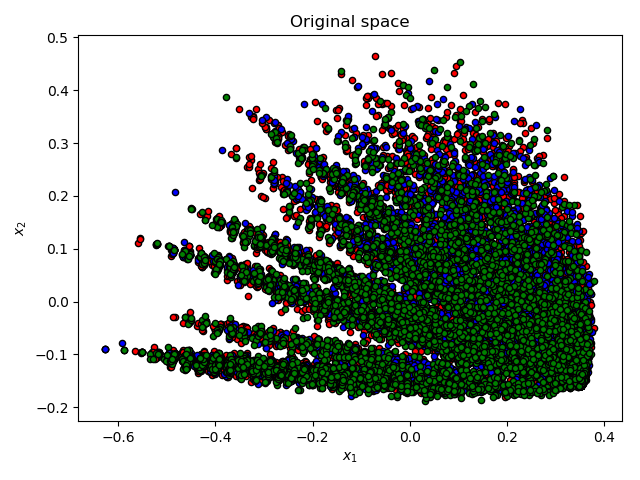
\includegraphics[width=\columnwidth]{Figures/Extensions/kPCALemmaRBF.png}
    \caption{kPCA performed on a Lemma Count Vectoriser using RBF kernel and a gamma of 0.04}
    \label{fig:balance}
  \end{figure}
  
